\documentclass[12pt]{article}
  
  \usepackage[utf8]{inputenc}
  \usepackage[T1]{fontenc}
  \usepackage{geometry}
  \usepackage{graphicx}
  \geometry{a4paper}
  
  \usepackage[frenchb]{babel}
  
  \title{Assignment No. B8}
  \author{Roll no : 4430}
  \date{}
  
  \begin{document}
  \maketitle
  
\section{Problem Definition}
Write a program to implement SLR Parsing algorithm using python for the ordered input set
in XML\\
P -> E,\\
E-> E+T\\
E-> T\\
T-> T*F\\
T-> F\\
F -> (E)\\
F -> i\\

\section{Learning Objectives}

\begin{enumerate}
\item To understand various parsing techniques.
\item To implement SLR parsing using python.
\end{enumerate}



\section{Mathematical Model}
Let S be the system of soluion of given problem statement.\\
s=\{s,e,I,O,F,DD,NDD,Su,Fu \}\\\\
where,\\
s=start state ;\\
such that, y=\{represents grammar productions.\}\\\\
e=end state;\\\\
I =  represents set of input\\
I = \{fparsing table,terminals,non- terminals, production rules,input string\}\\\\
where,\\
producton rules =lhs $\rightarrow$  rhs\\\\ input string = [a-z]* ;\\\\ terminals =   [a-z]+ \\\\nonterminals =  [A-Z]+\\\\

O represents set of output\\
O = status\\
where,\\\\ status= \{accept , error\}\\\\

F=set of functions.\\
F=\{f1,f2,f3\}\\
where,\\\\

f1= f1 represents the function to accept parse table.\\
f1 = \{I $\mid$ I $\in$ parse Table\}\\
{parser table $\in$ [a-z]*,[A-Z]*,[0-9],[special chars]*(\}

f2= f2 represents the function to parse string\\
f2 = \{I $\mid$ I $\in$ parse string\}\\
\{parse string $\in$ [a-z]*,[A-Z]*,[0-9]\}

f3= f3 to display the result of acceptance.\\
f3 = \{O $\mid$ if S $\in$ \{ f1,f2\} O $\in$ Su else O $\in$ Fu\}\\\\

DD = Deterministic Data\\
= parsing table\\\\

NDD (Non Deterministic Data)\\
= result of parsing\\\\

Sc =Success case\\ input string is accepted\\\\
Fc = Failure Case\\parse table does not have entry while parsing string\\\\

\section{Concept Related Theory}
\subsection{Parsing}
Every programming languages has a set of rules that must be followed by the programmer
and it is called as the syntax of the language.\\
So its the compiler duty to check if the programmer has followed the rule of the language.
The second phase of the compiler is assigned the task of checking the syntax
and thus it is called syntax analyser and parser.\\
It takes the input from a lexical analyser in the form of token streams.\\
The parser analyzes the source code (token stream) against the production rules to
detect any errors in the code. The output of this phase is a parse tree.\\
This way, the parser accomplishes two tasks, i.e., parsing the code, looking for errors
and generating a parse tree as the output of the phase.\\

\subsection{Parsing Strategies:}
Syntax analyzers follow production rules defined by means of context-free grammar.
The way the production rules are implemented (derivation) divides parsing into two types :
top-down parsing and bottom-up parsing.\\\\

\subsection{Bottom up Parsing technique:}
In bottom parsing start with the input string and try to obtain the starting symbol of the
grammar given using successive reductions.\\
Bottom-up parser considers the right most derivation of the input string.\\
In bottom-up parsing we can create a parse tree from leaves and proceeds towards the
root, which is attempting to construct the parse tree in the bottom-up.\\\\

SLR(1) are the Simple LR easiest to implement but weak in terms of the members of the
grammar in which it exceeds.\\
Parsing tables are constructed by this method is called as SLR table.\\
LR(0) items :\\
A LR(0)item of a grammar G is the production of G eith the dot at some position of
the right side. Thus the production A! XYZ yields the four items.\\
A -> . XYZ\\
A -> X . YZ\\
A -> XY . Z\\
A -> XYZ .\\
The production A generates A.\\
To find of the states of the SLR parser, we group items into sets called canonical LR(0).
We define an augmented grammar and two functions, closure and goto.\\
Augmented grammar is the grammar G with new introduced non terminal S’ and the
production S’ S. The production S’ S is introduced to indicate the parsing and
announce the acceptance of input.\\
Algorithm for SLR Parsing table :\\
Input : An augmented grammar G’.\\
Output : The SLR parsing table functions action and goto for G’.\\

\section{State Diagram }
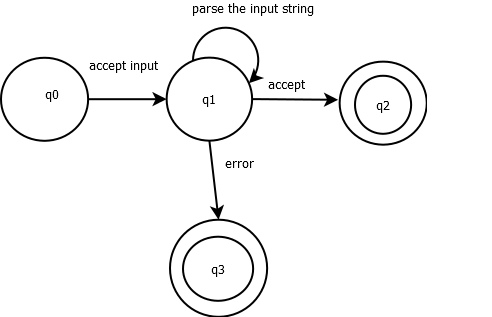
\includegraphics{b8state}

\section{Program Code and Output}
\begin{verbatim}
import xml.etree.ElementTree as ET

tree= ET.parse('parsing_table.xml')
root=tree.getroot()
term=[]
non_term=[]
lsprod=[]
rsprod=[]
n=0    #no of states
for child in root:
   if(child.tag=="states"):
      n=int(child.text)
   elif(child.tag=="term"):
      term.append(child.text)
   elif(child.tag=="nterm"):
      non_term.append(child.text)
   elif(child.tag=="productions"):
        for ch in child:
          lsprod.append(ch[0].text)
          rsprod.append(ch[1].text)
   elif(child.tag=="actiontable"):
      action=[[] for x in range(n)]
      i=0
      for ch in child:
         for c in ch:
           action[i].append(c.text)
         i=i+1

   elif(child.tag=="gototable"):
      goto=[[] for x in range(n)] 
      i=0
      for ch in child:
         for c in ch:
            goto[i].append(c.text)
         i=i+1

nterm=len(term)
nnterm=len(non_term)
nprod=len(lsprod)
print("Terminals:    "),;print(term)
print("Non Terminals:    "),;print(non_term)
print("Grammar Productions are as follows:   ")
for i in range(nprod):
   print(lsprod[i]+" -> "+rsprod[i])
print("\nAction Table:  ")
for i in range(n):
  print("")
  for j in range(nterm):
     print(action[i][j]+"   "),
print("")
print("Goto Table:    ")
for i in range(n):
  print(" ")
  for j in range(nnterm):
    print(str(goto[i][j])+"   "),

while True:
  #print("\nEnter input String:  "),
  istr=raw_input("\nEnter input String:  ")
  iptr=0
  #istr = 'abab'
  stack=['$',0]
  while True:
    print("Stack :"),
    print(stack)
    stop=stack[len(stack)-1]
    isym=istr[iptr]
    isindex=term.index(isym)
    ac=action[stop][isindex]
    print("Action for stop="+str(stop)+" and input symbol index"+
    str(isindex)+" is "+action[stop][isindex])
    if(ac=="Error"):
       print("Syntax Error!!!")
       break
    elif(ac=="Accept"):
       print("Correct Syntax!!")
       break
    elif("s" in ac):
       stack.append(isym)
       ns=ac.replace("s","")
       stack.append(int(ns))
       iptr=iptr+1
    elif("r" in ac):
       rrule=int(ac.replace("r",""))
       print("Reduce using rule  "+lsprod[rrule-1]+"  ->  "+rsprod[rrule-1])
       for i in range(2*len(rsprod[rrule-1])):
           stack.pop()
       print(stack)
       stack.append(lsprod[rrule-1])
       pstate=stack[len(stack)-2]
       ntindex=non_term.index(lsprod[rrule-1])
       nst=goto[pstate][ntindex]
       stack.append(int(nst))
       print(stack)

******************** PARSE FILE *********************

<parsetable>
    <states>8</states>
    <term>a</term>
    <term>b</term>
    <term>$</term>
    <nterm>S</nterm>
    <nterm>A</nterm>
    <productions>
         <prod><l>S</l><r>AS</r></prod>
         <prod><l>S</l><r>b</r></prod>
         <prod><l>A</l><r>SA</r></prod>
         <prod><l>A</l><r>a</r></prod>
    </productions>
    <actiontable>
        <tr><td>s5</td><td>s3</td><td>Error</td></tr>
        <tr><td>Error</td><td>Error</td><td>Accept</td></tr>
        <tr><td>s5</td><td>s3</td><td>Error</td></tr>
        <tr><td>r2</td><td>r2</td><td>r2</td></tr>
        <tr><td>s5</td><td>Error</td><td>Error</td></tr>
        <tr><td>r4</td><td>r4</td><td>Error</td></tr>
        <tr><td>r1</td><td>r1</td><td>r1</td></tr>
        <tr><td>r3</td><td>r3</td><td>Error</td></tr>
        
    </actiontable>
    <gototable>
        <tr><td>1</td><td>2</td></tr>
        <tr><td>0</td><td>0</td></tr>
        <tr><td>6</td><td>2</td></tr>
        <tr><td>0</td><td>0</td></tr>
        <tr><td>4</td><td>7</td></tr>
        <tr><td>0</td><td>0</td></tr>
        <tr><td>0</td><td>0</td></tr>
        <tr><td>0</td><td>0</td></tr>
    </gototable>
</parsetable>

***************************** OUTPUT **************************

ameeth@ubuntu-16.0.4:~/CL1$ python parse1.py
Terminals:     ['a', 'b', '$']
Non Terminals:     ['S', 'A']
Grammar Productions are as follows:   
S -> AS
S -> b
A -> SA
A -> a

Action Table:  

s5    s3    Error    
Error    Error    Accept    
s5    s3    Error    
r2    r2    r2    
s5    Error    Error    
r4    r4    Error    
r1    r1    r1    
r3    r3    Error    
Goto Table:    
 
1    2     
0    0     
6    2     
0    0     
4    7     
0    0     
0    0     
0    0    
Enter input String:  ab$
Stack : ['$', 0]
Action for stop=0 and input symbol index   0 is s5
Stack : ['$', 0, 'a', 5]
Action for stop=5 and input symbol index   1 is r4
Reduce using rule  A  ->  a
['$', 0]
['$', 0, 'A', 2]
Stack : ['$', 0, 'A', 2]
Action for stop=2 and input symbol index   1 is s3
Stack : ['$', 0, 'A', 2, 'b', 3]
Action for stop=3 and input symbol index   2 is r2
Reduce using rule  S  ->  b
['$', 0, 'A', 2]
['$', 0, 'A', 2, 'S', 6]
Stack : ['$', 0, 'A', 2, 'S', 6]
Action for stop=6 and input symbol index   2 is r1
Reduce using rule  S  ->  AS
['$', 0]
['$', 0, 'S', 1]
Stack : ['$', 0, 'S', 1]
Action for stop=1 and input symbol index   2 is Accept
Correct Syntax!!

Enter input String:  abb$
Stack : ['$', 0]
Action for stop=0 and input symbol index   0 is s5
Stack : ['$', 0, 'a', 5]
Action for stop=5 and input symbol index   1 is r4
Reduce using rule  A  ->  a
['$', 0]
['$', 0, 'A', 2]
Stack : ['$', 0, 'A', 2]
Action for stop=2 and input symbol index   1 is s3
Stack : ['$', 0, 'A', 2, 'b', 3]
Action for stop=3 and input symbol index   1 is r2
Reduce using rule  S  ->  b
['$', 0, 'A', 2]
['$', 0, 'A', 2, 'S', 6]
Stack : ['$', 0, 'A', 2, 'S', 6]
Action for stop=6 and input symbol index   1 is r1
Reduce using rule  S  ->  AS
['$', 0]
['$', 0, 'S', 1]
Stack : ['$', 0, 'S', 1]
Action for stop=1 and input symbol index   1 is Error
Syntax Error!!!



\end{verbatim}

\section{Conclusion}
We have thus successfully implemented SLR parsing technique using Python.

\end{document}